\documentclass[11pt]{article}
\usepackage[margin=1.5in]{geometry}
\usepackage{amsmath}
\usepackage{amssymb}
\usepackage{amsbsy}
\usepackage{bbm}
\usepackage{url}
\usepackage{color}
\usepackage{float}
\usepackage{graphicx}
\usepackage{epstopdf}
\usepackage{fancyhdr}
\usepackage{enumerate}
\usepackage{enumitem}
\usepackage{tikz}
\usepackage[ruled,vlined]{algorithm2e}
\usepackage[colorlinks=true,urlcolor=blue]{hyperref}
\usepackage{tabularx}
\usepackage{booktabs}
\usepackage { amsmath, amssymb }
\usepackage[utf8]{inputenc}
\numberwithin{figure}{section}

\title{CS224W Homework 2}
\author{yeeboxie}

\newcommand{\Solution}[1]{{\medskip \color{red} \bf $\bigstar$~\sf \textbf{Solution}~$\bigstar$ \sf #1 } \bigskip}
% \newcommand{\Solution}[1]{}
\begin{document}

\maketitle

\section{Node Embeddings with TransE [21 points]}

While many real world systems are effectively modeled as graphs, graphs can be a cumbersome format for certain downstream applications, such as machine learning models. It is often useful to represent each node of a graph as a vector in a continuous low dimensional space. The goal is to preserve information about the structure of the graph in the vectors assigned to each node. For instance, the spectral embedding preserved structure in the sense that nodes connected by an edge were usually close together in the (one-dimensional) embedding $x$.\newline
\noindent Multi-relational graphs are graphs with multiple types of edges. They are incredibly useful for representing structured information, as in knowledge graphs. There may be one node representing “Washington, DC” and another representing “United States”, and an edge between them with the type “Is capital of”. In order to create an embedding for this type of graph, we need to capture information about not just which edges exist, but what the types of those edges are. In this problem, we will explore a particular algorithm designed to learn node embeddings for multi-relational graphs. \newline
The algorithm we will look at is TransE.\footnote{See the 2013 NeurIPS paper by Bordes et al: \url{https://papers.nips.cc/paper/5071-translating-embeddings-for modeling-multi-relational-data.pdf}} \newline
We will first introduce some notation used in the paper describing this algorithm.
We’ll let a multi-relational graph $G = (E, S, L)$ consist of the set of \textit{entities} $E$ (i.e., nodes), a set of edges $S$, and a set of possible relationships $L$.
The set $S$ consists of triples $(h, l, t)$, where $h \in E$ is the \textit{head} or source-node, $l \in L$ is the relationship, and $t \in E$ is the \textit{tail} or destination-node.
As a node embedding, TransE tries to learn embeddings of each entity $e \in E$ into $\mathbb{R}^k$ ( $k$-dimensional vectors), which we will notate by $\mathbf{e}$. The main innovation of TransE is that each relationship $\ell$ is also embedded as a vector $\ell \in \mathbb{R}^k$, such that the difference between the embeddings of entities linked via the relationship $\ell$ is approximately $\ell$. That is, if $(h, \ell, t) \in S$, TransE tries to ensure that $\mathbf{h}+\boldsymbol{\ell} \approx \mathbf{t}$. Simultanesouly, TransE tries to make sure that $\mathbf{h}+\boldsymbol{\ell} \not\approx \mathbf{t}$ if the edge $(h, \ell, t)$ does not exist.\newline
\textbf{Note on notation}: we will use unbolded letters $e, \ell$, etc. to denote the entities and relationships in the graph, and bold letters $\mathbf{e}, \boldsymbol{\ell}$, etc., to denote their corresponding embeddings.
TransE accomplishes this by minimizing the following loss:
\begin{equation}\label{eq1}
\mathcal{L}=\sum_{(h, \ell, t) \in S}\left(\sum_{\left(h^{\prime}, \ell, t^{\prime}\right) \in S_{(h, \ell, t)}^{\prime}}\left[\gamma+d(\mathbf{h}+\boldsymbol{\ell}, \mathbf{t})-d\left(\mathbf{h}^{\prime}+\boldsymbol{\ell}, \mathbf{t}^{\prime}\right)\right]_{+}\right)
\end{equation}
Here $\left(h^{\prime}, \ell, t^{\prime}\right)$ are "corrupted" triplets, chosen from the set $S_{(h, \ell, t)}^{\prime}$ of corruptions of $(h, \ell, t)$, which are all triples where either $h$ or $t$ (but not both) is replaced by a random entity, and $\ell$ remains the same as the one in the original triplets.
$$
S_{(h, \ell, t)}^{\prime}=\left\{\left(h^{\prime}, \ell, t\right) \mid h^{\prime} \in E\right\} \cup\left\{\left(h, \ell, t^{\prime}\right) \mid t^{\prime} \in E\right\}
$$
Additionally, $\gamma>0$ is a fixed scalar called the \textit{margin}, the function $d(\cdot, \cdot)$ is the Euclidean distance, and $[\cdot]_{+}$ is the positive part function (defined as $\max (0, \cdot)$). Finally, TransE restricts \textbf{all the entity embeddings to have length $1:\|\mathbf{e}\|_2=1$ for every $e \in E$.}\\
For reference, here is the TransE algorithm, as described in the original paper on page 3:
\begin{figure}[H]
    \centering
    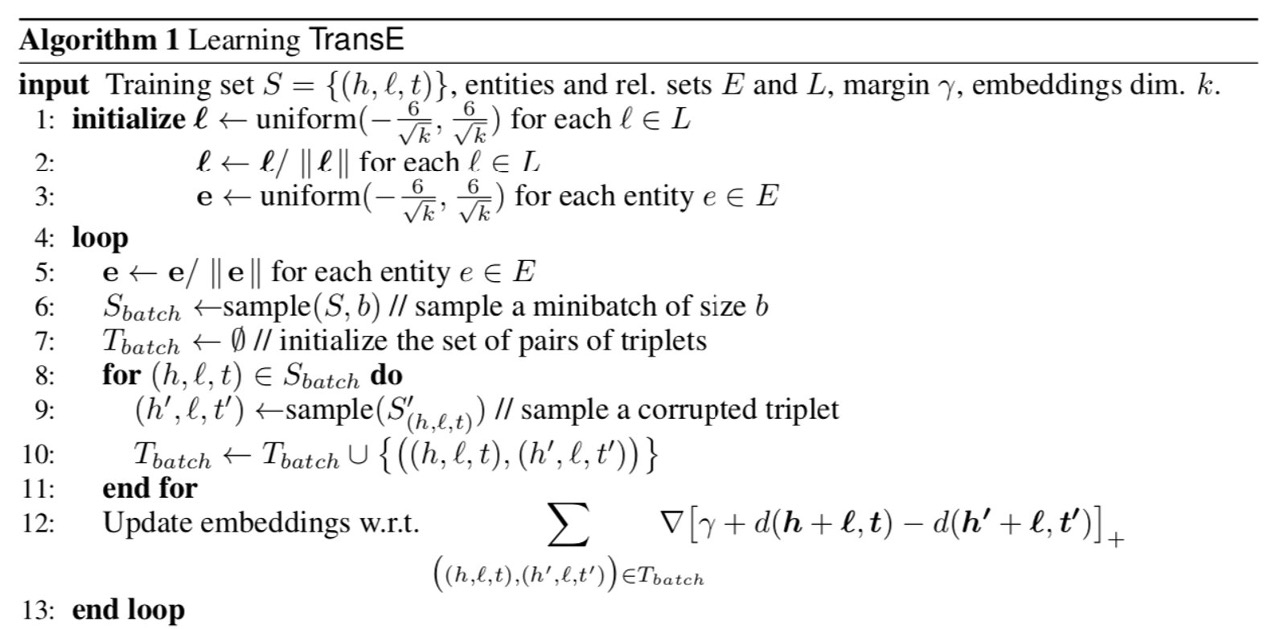
\includegraphics[width=1.0\textwidth]{CS224W_Homework2/algo2.png}
    \label{fig:algo2}
\end{figure}

\subsection{Simplified Objective [3 points]}
Say we were intent on using a simpler loss function. Our objective function (\ref{eq1}) includes a term maximizing the distance between $\mathbf{h}^{\prime}+\boldsymbol{\ell}$ and $\mathbf{t}^{\prime}$. If we instead simplified the objective, and just tried to minimize
\begin{equation}\label{eq2}
\mathcal{L}_{\text {simple }}=\sum_{(h, \ell, t) \in S} d(\mathbf{h}+\boldsymbol{\ell}, \mathbf{t}),
\end{equation}

we would obtain a useless embedding. Give an example of a simple graph and corresponding embeddings which will minimize the new objective function (\ref{eq2}) all the way to zero, but still give a completely useless embedding.\\
\textbf{Hint:} Your graph should be non-trivial, i.e., it should include at least two nodes and at least one edge. Assume the embeddings are in 2 dimensions, i.e., $k = 2$.
What happens if $\boldsymbol{\ell} = \textbf{0}$?

\Solution{}

We can embed all the entities with $\left(0,1\right)$ and get the minimum loss function value of $0$ although this kind of embeding is useless.

\subsection{Utility of $\gamma$  [5 points]}
We are interested in understanding what the margin term $\gamma$ accomplishes. If we removed the margin term $\gamma$ from our loss, and instead optimized
\begin{equation}\label{eq3}
\mathcal{L}_{\text {no margin }}=\sum_{(h, \ell, t) \in S} \sum_{\left(h^{\prime}, \ell t^{\prime}\right) \in S_{(h, \ell, t)}^{\prime}}\left[d(\mathbf{h}+\boldsymbol{\ell}, \mathbf{t})-d\left(\mathbf{h}^{\prime}+\boldsymbol{\ell}, \mathbf{t}^{\prime}\right)\right]_{+},
\end{equation}
it turns out that we would again obtain a useless embedding. Give an example of a simple graph and corresponding embeddings which will minimize the new objective function (\ref{eq3}) all the way to zero, but still give a completely useless embedding. By useless, we mean that in your example, you cannot tell just from the embeddings whether two nodes are linked by a particular relation (Note: your graph should be non-trivial, i.e., it should include at least two nodes and at least one edge. Assume the embeddings are in 2 dimensions, i.e., $k=2$.)

\Solution{}

We can embed all the entities with $\left(0,1\right)$ and get the minimum loss function value of $0$ although this kind of embeding is useless.

Without $\gamma$, the loss function does not enforce a sufficient gap between positive and negative pairs, allowing the embeddings to be degenerate. Even though the loss function reaches zero, the embeddings may not encode any meaningful relational information, making them "useless" in practice.

\subsection{ Normalizing the embeddings [5 points]}
Recall that TransE normalizes every entity embedding to have unit length (see line 5 of the algorithm). The quality of our embeddings would be much worse if we did not have this step. To understand why, imagine running the algorithm with line 5 omitted.
What could the algorithm do to trivially minimize the loss in this case? What would the embeddings
it generates look like?

\Solution{}

Without the normalization step, the embeddings could look like the following:

\begin{enumerate}[label=\textbullet, left=2em]
    \item Arbitrary scaling: The embeddings could become arbitrarily large. For instance, instead of embeddings like $h=\left(0.5,0.3\right)$, you could end up with h=(10,6). While this might still respect the relative distances (i.e., $d\left(h,t\right)$ might remain the same), the actual embeddings would be unnecessarily large, leading to poor generalization and lack of structure in the learned representation.

    \item Identical embeddings: The embeddings of all entities might collapse into a single point, e.g., $h=t=h^{\prime} =t^{\prime}=\left(0,0\right)$. This would trivially minimize the loss by making all distances zero, but it would obviously result in useless embeddings for distinguishing relationships.
\end{enumerate}



\subsection{Expressiveness of TransE embeddings [8 points]}
Give an example of a simple graph for which no perfect embedding exists, i.e., no embedding perfectly satisfies $\mathbf{u}+\boldsymbol{\ell}=\mathbf{v}$ for all $(u, \ell, v) \in S$ and $\mathbf{u}+\boldsymbol{\ell} \neq \mathbf{v}$ for $(u, \ell, v) \notin S$, for any choice of entity embeddings ($\mathbf{e}$ for $e \in E$ ) and relationship embeddings ( $\boldsymbol{\ell}$ for $\ell \in L$ ). Explain why this graph has no perfect embedding in this system, and what that means about the expressiveness of TransE embeddings. As before, assume the embeddings are in 2 dimensions $(k=2)$.\\
\textbf{Hint: }By expressiveness of TransE embeddings, we want you to talk about which type of relationships TransE can/cannot model with an example. (Note that the condition for this question is slightly different from that for Question 2.1 and what we ask you to answer is different as well).

\Solution{}
TransE struggles with modeling \textbf{1-n (one-to-many)} and \textbf{symmetric relations} due to its simplistic approach.

\textbf{1-n (One-to-Many) Relations}

In a one-to-many relation, one entity (the head) is connected to multiple entities (the tails). For example, consider the relation ``author of'':
$$
\text{``J.K. Rowling''} \xrightarrow{\text{author of}} \text{``Harry Potter''}
$$
$$
\text{``J.K. Rowling''} \xrightarrow{\text{author of}} \text{``Fantastic Beasts''}
$$

For TransE to model this correctly, it needs to learn that the vector for ``J.K. Rowling'' plus the relation vector for ``author of'' should match different tail vectors, such as ``Harry Potter'' and ``Fantastic Beasts.'' However, because TransE represents relations as translations, it assumes that the relation vector remains constant. This is problematic because one relation cannot simultaneously map to multiple different tail entities in the same way, making it difficult for TransE to handle one-to-many relations properly.

\textbf{Symmetric Relations}

For symmetric relations, the order of the entities doesn't matter. For example, consider the relation ``is friend of'':
$$
\text{``Alice''} \xrightarrow{\text{is friend of}} \text{``Bob''}
$$
$$
\text{``Bob''} \xrightarrow{\text{is friend of}} \text{``Alice''}
$$

In this case, the relationship between Alice and Bob is bidirectional, meaning if the triplet $(\text{Alice}, \text{is friend of}, \text{Bob})$ holds true, so does \((\text{Bob}, \text{is friend of}, \text{Alice})\).

However, TransE models the relation $r$ as a translation, so it expects that $h + r \approx t$. This implies that for a symmetric relation, the vectors for \(h\) and \(t\) should be identical, or the relation vector \(r\) should be zero (i.e., no translation), which contradicts the assumption of a non-zero relation vector for the translation. Thus, TransE struggles to model symmetric relations effectively because it cannot capture the bidirectionality properly.

\textbf{Summary}

\begin{itemize}
    \item \textbf{1-n relations}: TransE cannot handle these well because it assumes a fixed translation for a relation, which fails when one entity is connected to multiple others.
    \item \textbf{Symmetric relations}: TransE cannot handle these effectively because it assumes a directional translation, which conflicts with the bidirectionality inherent in symmetric relations.
\end{itemize}

These limitations highlight why more advanced models like TransH or TransR, which introduce more flexibility in representing relations, are often preferred for handling such cases.

\newpage

\section{Expressive Power of Knowledge Graph Embeddings [10 points]}
TransE is a common method for learning representations of entities and relations in a knowledge graph. Given a triplet $(h, \ell, t)$, where entities embedded as $h$ and $t$ are related by a relation embedded as $\ell$, TransE trains entity and relation embeddings to make $h+\ell$ close to $t$. There are some common patterns that relations form:
\begin{itemize}
    \item Symmetry: A is married to B, and B is married to A.
    \item Inverse: A is teacher of B, and B is student of A. Note that teacher and student are 2 different relations and have their own embeddings.
    \item Composition: $\mathrm{A}$ is son of $\mathrm{B} ; \mathrm{C}$ is sister of $\mathrm{B}$, then $\mathrm{C}$ is aunt of $\mathrm{A}$. Again note that son, sister, and aunt are 3 different relations and have their own embeddings.
\end{itemize}
\subsection{TransE Modeling [3 points]}
For each of the above relational patterns, can TransE model it perfectly, such that $h+\ell=t$ for all relations? Explain why or why not. Note that here $\mathbf{0}$ embeddings for relation are undesirable since that means two entities related by that relation are identical and not distinguishable.

\Solution{}
\begin{enumerate}[label=\textbullet]
    \item \textbf{Symmetry}: TransE cannot model symmetric relations perfectly. For a symmetric relation $\ell$, both $\left(h,\ell,t\right)$ and $\left(t,\ell,h\right)$ must hold, implying $h+\ell \approx t$ and $t+\ell \approx h$. Adding these equations gives $2\ell \approx 0$, forcing $\ell \approx 0$. However, a zero relation embedding is undesirable, as it collapses $h$ and $t$ into the same vector, making them indistinguishable. Thus, symmetry cannot be modeled without violating the non-zero constraint.
    \item \textbf{Inverse}: TransE can model inverse relations. If $\ell_{1}$ and $\ell_{2}$ are inverses (e.g., "teacher" and "student"), then $\left(h,\ell_{1},t\right)$ implies $h+\ell_{1} \approx t$ and $\left(t,\ell_{2},h\right)$ implies $t+\ell_{2} \approx h$. Substituting the first into the second gives $\ell_{1} + \ell_{2} \approx 0$, meaning $\ell_{2} \approx \neg\ell_{1}$. This allows distinct non-zero embeddings for $\ell_{1}$ and $\ell_{2}$ while preserving invertibility.
    \item \textbf{Composition} TransE can model compositional relations. Suppose $(h,\ell_{1},t_{1})$ and $(t_{1},\ell_{2},t)$ imply $(h,\ell_{3},t)$. TransE enforces $h+\ell_{1} \approx t_{1}$ and $t_{1}+\ell_{2} \approx t$,leading to $h+\ell_{1}+\ell_{2} \approx t$. If $\ell_{3}=\ell_{1}+\ell_{2}$, the composition holds. For example, if "son" $(\ell_{1})$ and "sister" $(\ell_{2})$ compose to "aunt" $(\ell_{3})$, TransE can learn $\ell_{3} \approx \ell_{2} - \ell_{1}$ (since $t_{1}=h+\ell_{1}$ and $t=t_{1}+\ell_{2}=h+\ell_{1}+\ell_{2})$. Thus, composition is achievable through linear combinations of relation vectors.
\end{enumerate}

\textbf{Summary}:
\begin{enumerate}
    \item Symmetry: No (requires zero relation embedding).
    \item Inverse: Yes (via negation).
    \item Composition: Yes (via additive relation embeddings).
\end{enumerate}

\subsection{RotatE Modeling [3 points]}
Consider a new model, RotatE. Instead of training embeddings such that $h+\ell \approx t$, we train embeddings such that $h \circ \ell \approx t$. Here $\circ$ means rotation. You can think of $h$ as a vector of dimension $2 d$, representing $d$ $2 \mathrm{D}$ points. $\ell$ is a $d$-dimensional vector specifying rotation angles. When applying $\circ$, For all $i \in 0 \ldots d-1, \left(h_{2 i}, h_{2 i+1}\right)$ is rotated clockwise by $l_i$. Similar to TransE, the entity embeddings are also normalized to L2 norm 1. Can RotatE model the above 3 relation patterns perfectly? Why or why not?

\Solution{}

RotatE can model all three relational patterns (symmetry, inverse, and composition) \textbf{perfectly}, unlike TransE. Here's why:

\subsection*{1. Symmetry}
\textbf{Example}: ``A is married to B'' and ``B is married to A.''
\begin{itemize}
    \item \textbf{Mechanism}: A symmetric relation requires $h \circ \ell \approx t$ and $t \circ \ell \approx h$.
    \item \textbf{Solution}: RotatE uses a rotation angle $\ell = \pi$ (180$^\circ$). Rotating $h$ by $\pi$ gives $t$, and rotating $t$ by $\pi$ recovers $h$:
    \[
    h \circ \pi \approx t \quad \text{and} \quad t \circ \pi \approx h.
    \]
    This satisfies symmetry without collapsing embeddings (unlike TransE’s zero-vector issue).
    \item \textbf{Why it works}: Rotations by $\pi$ flip the vector direction while preserving its norm (L2=1).
\end{itemize}

\subsection*{2. Inverse}
\textbf{Example}: ``A is teacher of B'' ($\ell_1$) and ``B is student of A'' ($\ell_2$).
\begin{itemize}
    \item \textbf{Mechanism}: Inverse relations require $h \circ \ell_1 \approx t$ and $t \circ \ell_2 \approx h$.
    \item \textbf{Solution}: Set $\ell_2 = -\ell_1$ (negative angle). Rotating $t$ by $-\ell_1$ cancels the original rotation:
    \[
    h \circ \ell_1 \approx t \quad \Rightarrow \quad t \circ (-\ell_1) \approx h.
    \]
    \item \textbf{Why it works}: Rotations are invertible via angle negation, preserving distinct embeddings for both relations.
\end{itemize}

\subsection*{3. Composition}
\textbf{Example}: ``A is son of B'' ($\ell_1$), ``C is sister of B'' ($\ell_2$), so ``C is aunt of A'' ($\ell_3$).
\begin{itemize}
    \item \textbf{Mechanism}: Composition requires $h \circ \ell_1 \circ \ell_2 \approx t$ for $\ell_3 = \ell_1 + \ell_2$.
    \item \textbf{Solution}: Define $\ell_3$ as the sum of angles from $\ell_1$ and $\ell_2$. For instance:
    \[
    \text{Parent: } \ell_{\text{parent}} = -\ell_{\text{son}}, \quad \text{Aunt: } \ell_{\text{aunt}} = \ell_{\text{sister}} + \ell_{\text{parent}}.
    \]
    This ensures $h \circ \ell_{\text{aunt}} \approx t$ through additive angle composition.
    \item \textbf{Why it works}: Rotations are closed under addition (angles compose linearly), enabling hierarchical relationships.
\end{itemize}

\subsection*{Key Strengths of RotatE}
\begin{itemize}
    \item \textbf{Non-Collapsing Embeddings}: Normalization to L2=1 ensures entities remain distinct after rotation.
    \item \textbf{Rotation Invariance}: Rotations preserve vector norms, avoiding TransE’s limitations with symmetric relations.
    \item \textbf{Flexibility}: Angles can represent complex relational patterns (e.g., inverse via negation, composition via addition).
\end{itemize}

\textbf{Conclusion}: RotatE successfully models symmetry, inverse, and composition by leveraging rotational transformations, which are inherently reversible and composable.


\subsection{Failure Cases [4 points]}
Give an example of a graph that RotatE cannot model perfectly. Can TransE model this graph perfectly? Assume that relation embeddings cannot be $\mathbf{0}$ in either model.

\Solution{}
\section*{Answer}

Consider a graph with the following entities and relation:
\begin{itemize}
  \item Entities: 
    \begin{align*}
      A &= (1, 0, 0, 0) \quad (\text{normalized 4D vector}), \\
      B &= (0, 0, 1, 0) \quad (\text{normalized 4D vector}).
    \end{align*}
  \item Relation: $\ell$ such that $(A, \ell, B)$ holds.
\end{itemize}

\subsection*{Analysis for RotatE}
\begin{itemize}
  \item \textbf{Rotation Constraints}: 
    \begin{itemize}
      \item RotatE splits $A$ into two 2D components: $(1, 0)$ and $(0, 0)$. 
      \item Applying rotation angles $\ell_i$ to these components:
        \begin{align*}
          \text{First pair: } &(1, 0) \xrightarrow{\text{rotate } \ell_1} (\cos \ell_1, \sin \ell_1), \\
          \text{Second pair: } &(0, 0) \xrightarrow{\text{rotate } \ell_2} (0, 0).
        \end{align*}
    \end{itemize}
  \item \textbf{Failure}: The rotated result is $(\cos \ell_1, \sin \ell_1, 0, 0)$. To match $B = (0, 0, 1, 0)$, we need:
    \begin{align*}
      \cos \ell_1 = 0 \quad \text{and} \quad \sin \ell_1 = 0 \quad (\text{impossible}).
    \end{align*}
  \item \textbf{Key Issue}: RotatE cannot transfer magnitude between separate 2D planes.
\end{itemize}

\subsection*{Analysis for TransE}
\begin{itemize}
  \item \textbf{Translation}: 
    \begin{align*}
      A + \ell &= (1, 0, 0, 0) + (-1, 0, 1, 0) = (0, 0, 1, 0) = B.
    \end{align*}
  \item \textbf{Success}: The relation embedding $\ell = (-1, 0, 1, 0)$ is non-zero and valid. TransE freely redistributes magnitude across dimensions.
\end{itemize}

\subsection*{Conclusion}
\begin{itemize}
  \item RotatE fails because rotations are confined to individual 2D planes. 
  \item TransE succeeds because translations operate globally across dimensions.
\end{itemize}

\newpage

\section{Queries on Knowledge Graphs [14 points]}

Knowledge graphs (KGs) can encode a wealth of information about the world. Beyond representing the information using knowledge graphs, we can often derive previously unknown insights about entities and relations in the graphs. In this question, we will explore different approaches for reasoning over knowledge graphs. Recall from that lecture that we are interested in predicting \texttt{tail} nodes given (\texttt{head}, \texttt{relation}). We will use the same formulation throughout this question.


\subsection{Path Queries on Complete KGs [3 points]}
Consider the biomedicine knowledge graph from lecture. Assume the question of interest is: ``What proteins are associated with diseases treated by Arimidex?" Write the question in query form (eg. (e:AnchorEntity, (r:Relation))) and find the answer(s) to the query. Partial credit will be rewarded to correct intermediate steps.

\begin{figure}[H]
    \centering
    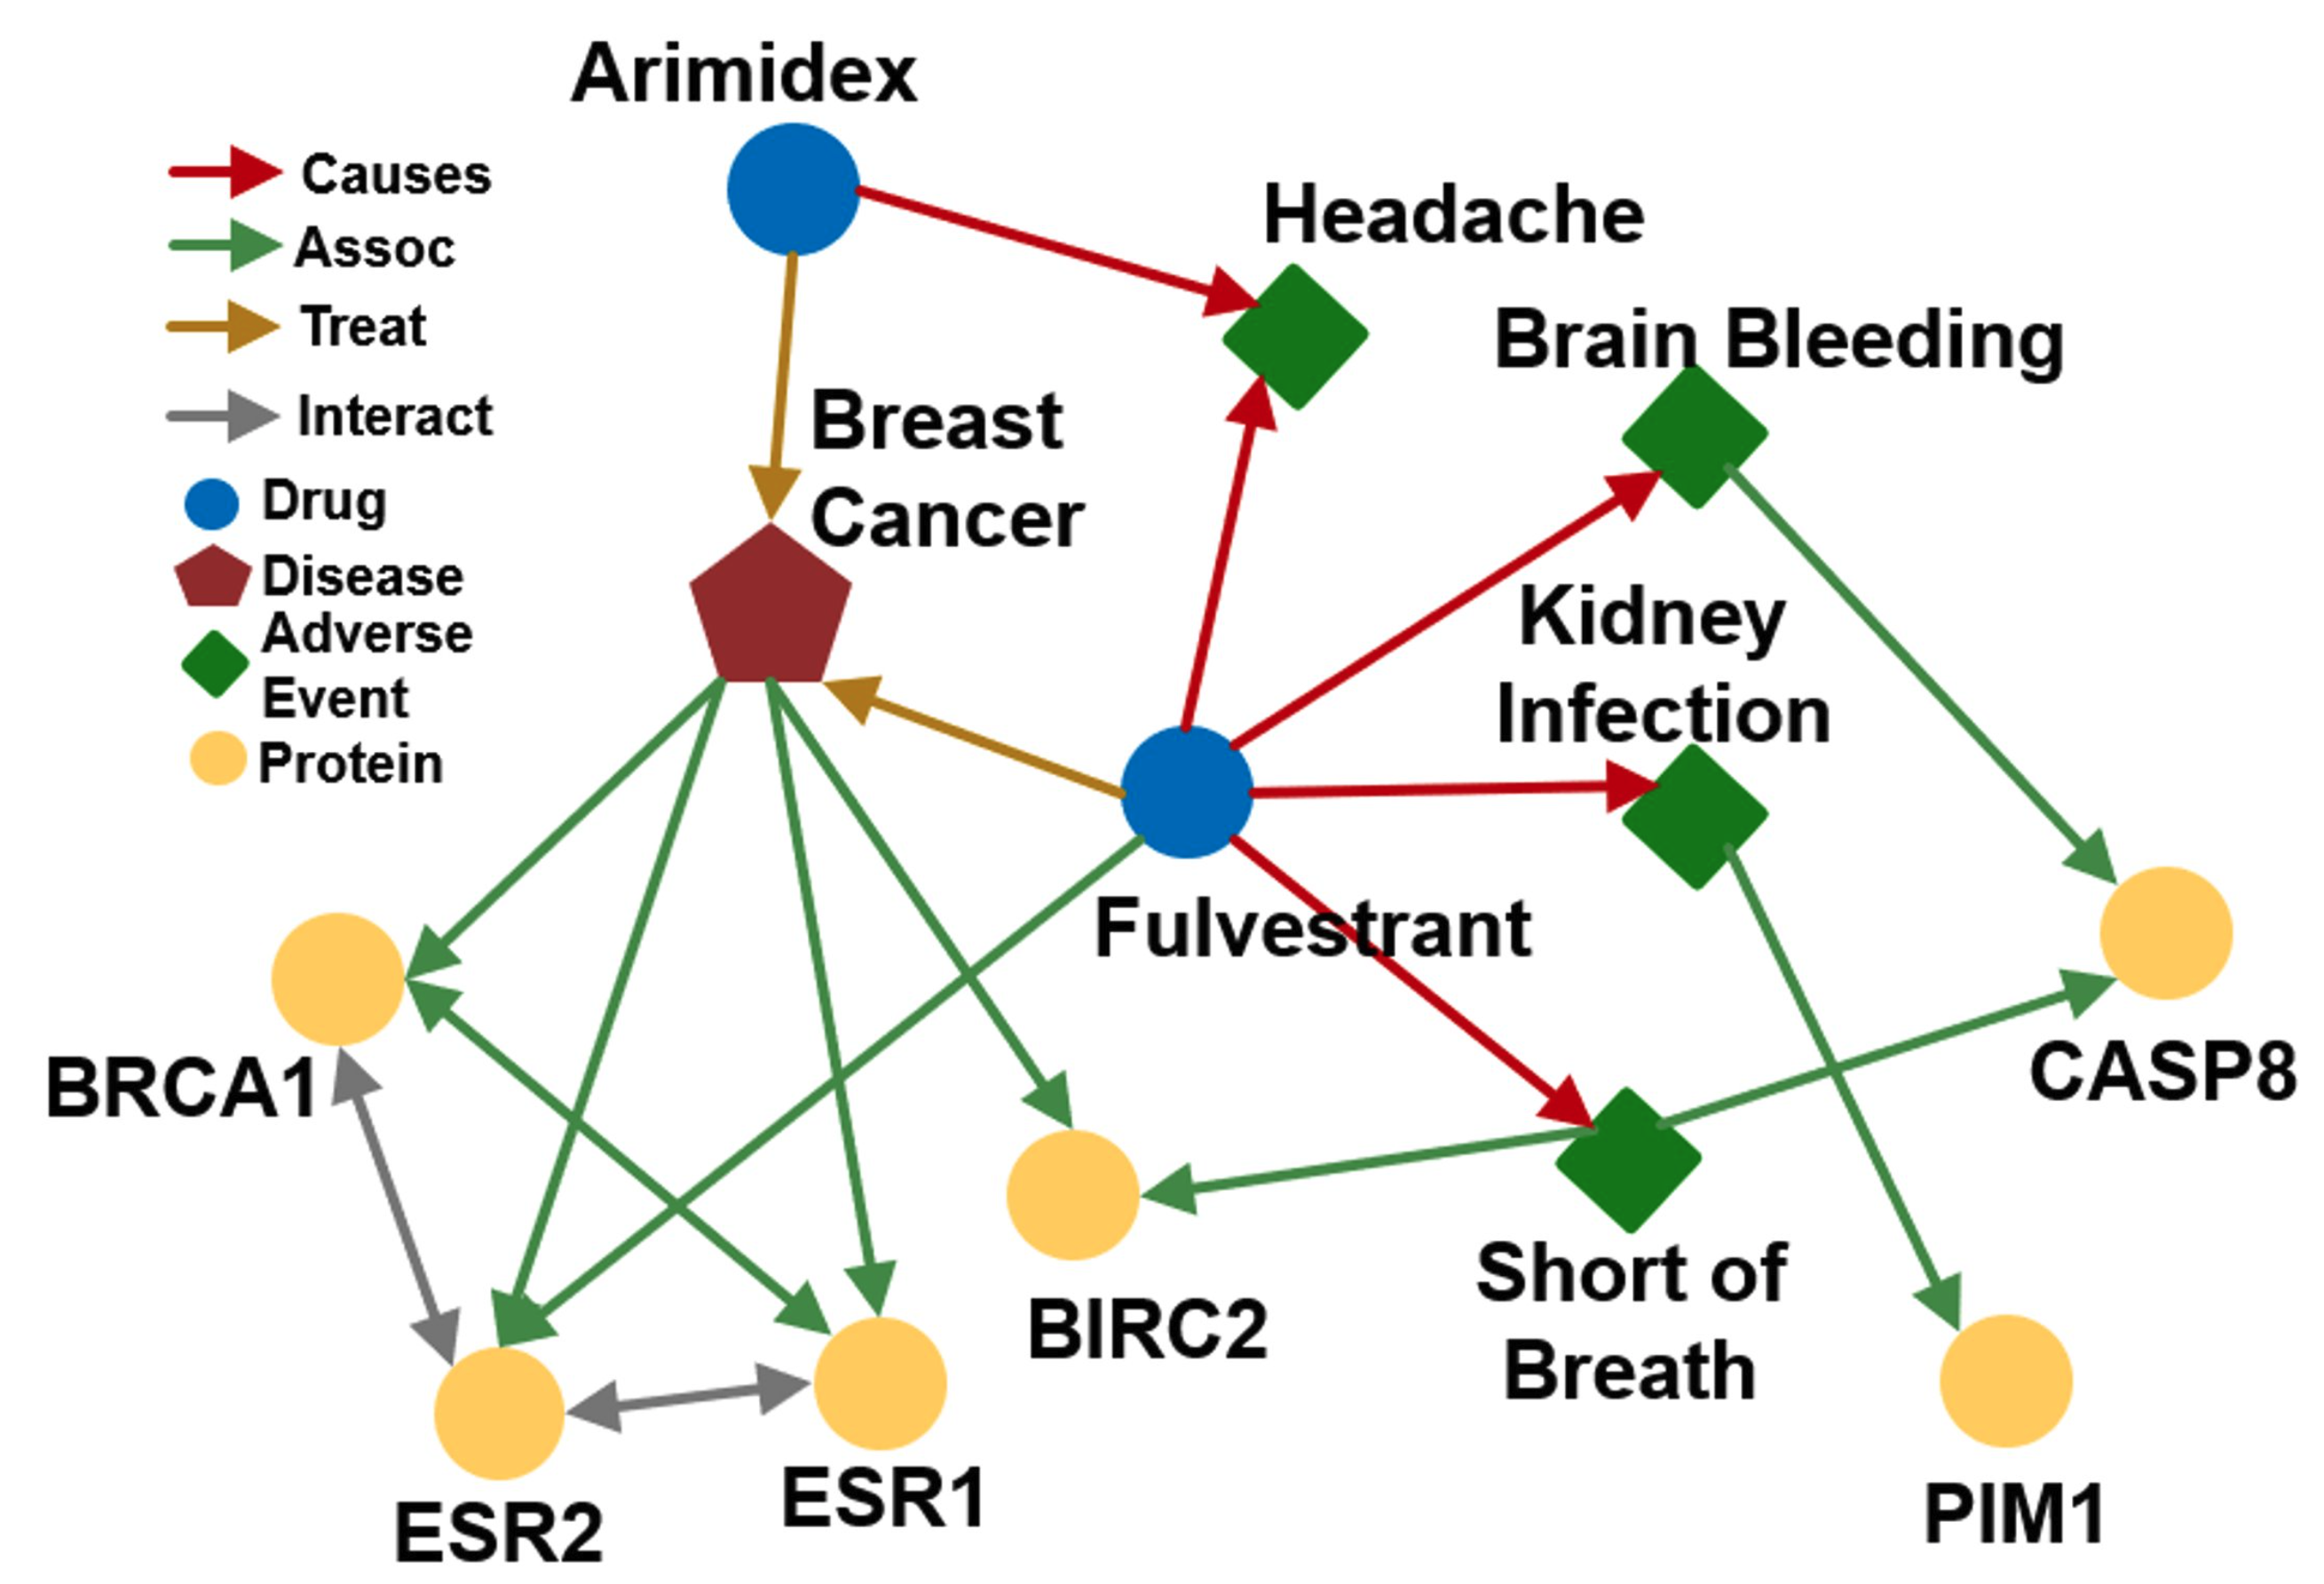
\includegraphics[width=0.8\textwidth]{CS224W_Homework2/5.1.png}
    \label{fig:5.1}
\end{figure}

\Solution{}

$\left( e: \text{Arimidex}, \left( r: \text{Treat}, r: \text{Assoc} \right)\right)$

$\text{ESR1}$


\subsection{Conjunctive Queries on Complete KGs [1 point]}
Consider the same biomedicine knowledge graph from before. Write a conjunctive query to which BIRC2 is the only answer using drugs as anchor entities. If such a query doesn't exist, provide a one-sentence explanation.

\Solution{}

What proteins are associated with Shortness of Breath caused by Fluvestrant and associated with Breast Cancer treated with Arimidex?

$\left((e: \text{Armidex}, (r: \text{Treat}, r: \text{Assoc})), (e: \text{Fulvestrant}, (r: \text{Cause}, r: \text{Assoc} ))  \right)$


\subsection{Incomplete KGs [2 points]}
A major issue with direct traversals on knowledge graphs is that they are usually incomplete in reality. One solution is to encode entities, relations, and queries in an embedding space that meaningfully organizes information. We would then be able to impute missing relation links by considering all nearby points of the query embedding as answers to the query. From lecture, we learned that TransE embeddings can be used for this. Can you come up with a way to adopt DistMult embeddings, which uses bilinear modeling, for answering path queries? If yes, describe in one or two sentences what can be modified from the TransE application. If no, provide a one-sentence explanation.

\Solution{}

Yes, DistMult can be adapted for path queries by replacing TransE's additive composition of relations with multiplicative composition (element-wise product of relation embeddings) along the path, followed by the bilinear scoring function to compute answer entity scores.


\subsection{Query2box [8 points]}

Query2box is an effective approach for answering complex conjunctive queries. Consider the following 2-dimensional embedding space. Assume that there are 7 entities $A, B, C, D, E, F, G \in V$, whose embeddings are shown below. There are 3 relations: $R_1, R_2, R_3$. $R_1 \in R$ shifts the center of a box by $(0.25, 2)$ and increases the width and height of a box by $(0.5, 2)$. $R_2$ shifts the center of a box by $(1, 0)$ and increases the width and height of a box by $(1, 0)$. $R_3$ shifts the center of a box by $(-0.75, 1)$ and increases the width and height of a box by $(1.5, 3)$.

Use the Query2box projection operator to find the answers to the conjunctive query: ((e:$A$, (r:$R_1$, r:$R_2$), (e:$C$, (r:$R_3$)). Show your work. Partial credit will be rewarded to correct intermediate steps.

Note: Shifting by a negative value means moving towards the left or bottom. Increasing the width and height by an amount means adding that amount in absolute value, not multiplying that amount as a factor. Assume that each path query starts with a box centered at the anchor entity with zero width and height.

\begin{figure}[H]
    \centering
    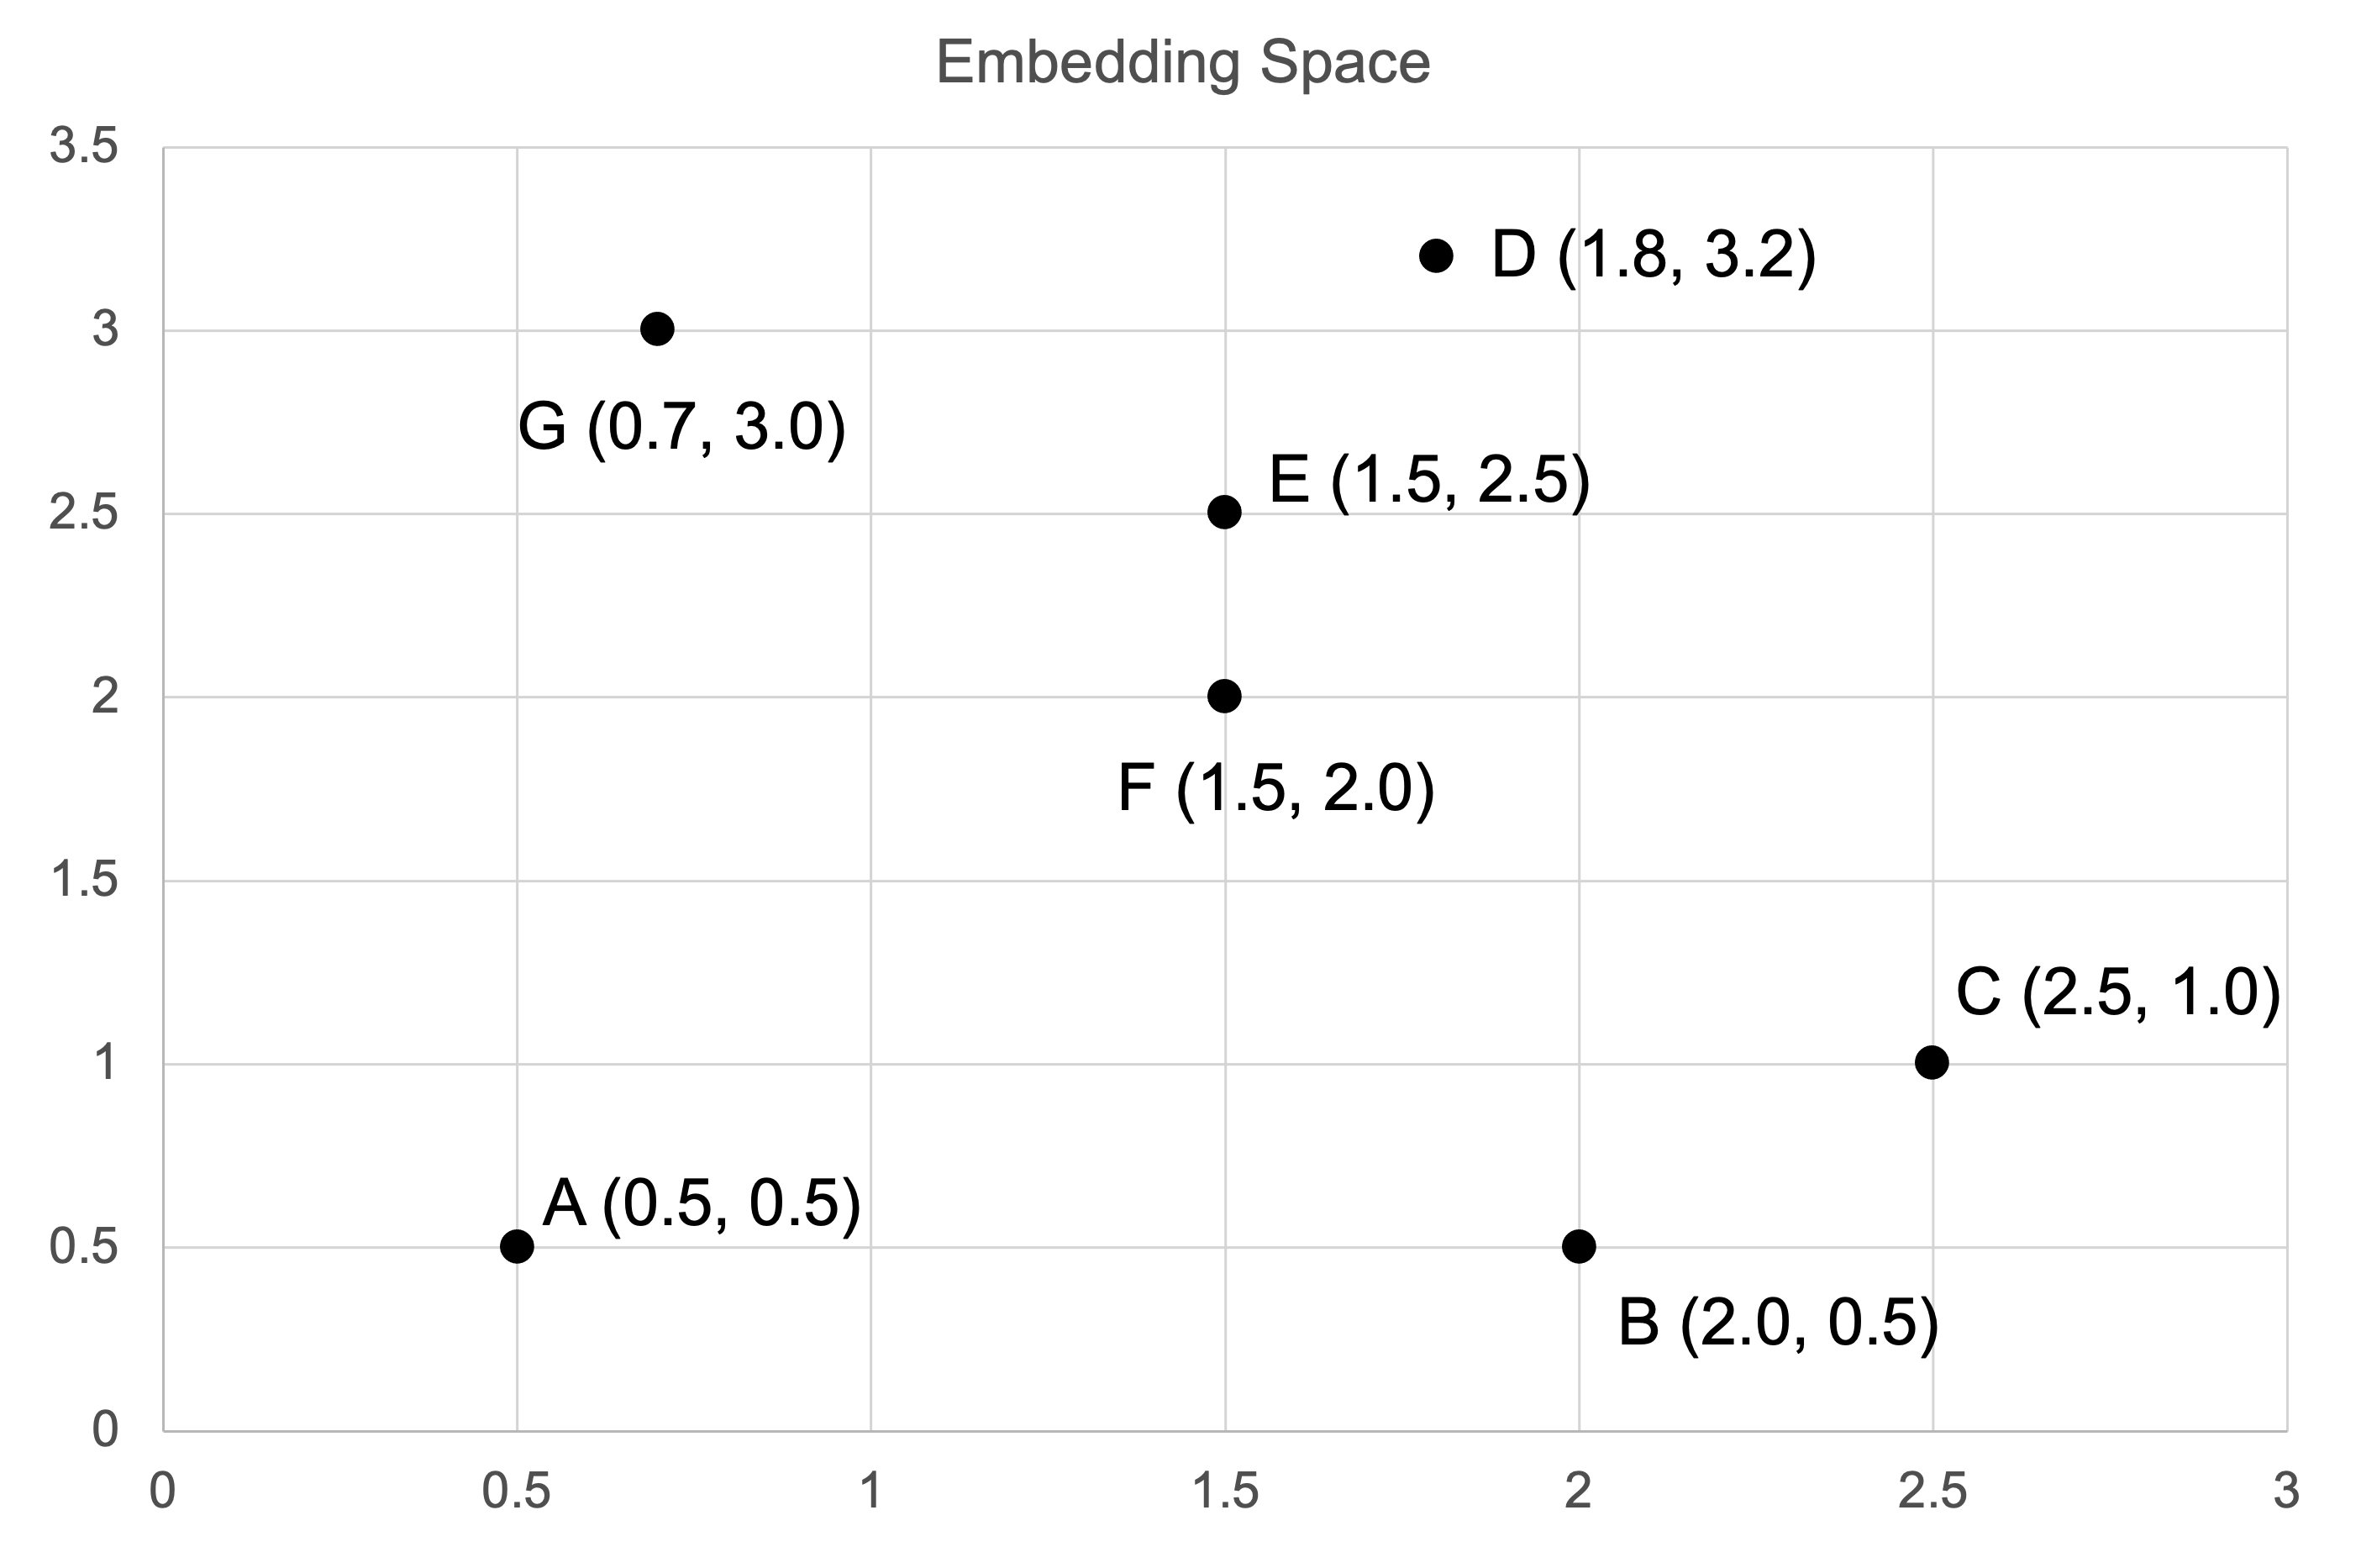
\includegraphics[width=0.9\textwidth]{CS224W_Homework2/5.4.png}
    \label{fig:5.4}
\end{figure}

\Solution{}

\subsection*{Step 1: Compute boxes for each path query}

\textbf{Path 1: }$(e:A, (r:R_1, r:R_2))$  
\begin{align*}
\text{Start: } & \text{Center } A = (0.5, 0.5),\ \text{Width}=0,\ \text{Height}=0 \\
\text{Apply } R_1: & \text{Center } = (0.5+0.25, 0.5+2) = (0.75, 2.5),\ \text{Width}=0.5,\ \text{Height}=2 \\
\text{Apply } R_2: & \text{Center } = (0.75+1, 2.5+0) = (1.75, 2.5),\ \text{Width}=1.5,\ \text{Height}=2 \\
\text{Final Box: } & X \in [1.75 - 0.75, 1.75 + 0.75] = [1.0, 2.5],\ Y \in [2.5 - 1.0, 2.5 + 1.0] = [1.5, 3.5]
\end{align*}

\textbf{Path 2: }$(e:C, (r:R_3))$  
\begin{align*}
\text{Start: } & \text{Center } C = (2.5, 1.0),\ \text{Width}=0,\ \text{Height}=0 \\
\text{Apply } R_3: & \text{Center } = (2.5-0.75, 1.0+1) = (1.75, 2.0),\ \text{Width}=1.5,\ \text{Height}=3 \\
\text{Final Box: } & X \in [1.75 - 0.75, 1.75 + 0.75] = [1.0, 2.5],\ Y \in [2.0 - 1.5, 2.0 + 1.5] = [0.5, 3.5]
\end{align*}

\subsection*{Step 2: Compute intersection of boxes}
$$
\begin{aligned}
&X\text{-overlap: } [\max(1.0, 1.0), \min(2.5, 2.5)] = [1.0, 2.5] \\
&Y\text{-overlap: } [\max(1.5, 0.5), \min(3.5, 3.5)] = [1.5, 3.5]
\end{aligned}
$$
\textbf{Intersection Box: }$X \in [1.0, 2.5],\ Y \in [1.5, 3.5]$

\subsection*{Step 3: Check entities within the intersection box}

\begin{tabularx}{\textwidth}{l|ll|cc|c}
\toprule
\textbf{Entity} & \textbf{Coordinates} & & \textbf{X in [1.0, 2.5]} & \textbf{Y in [1.5, 3.5]} & \textbf{In Intersection?} \\
\midrule
A & (0.5, 0.5) & & $\times$ & $\times$ & $\times$ \\
B & (2.0, 0.5) & & $\checkmark$ & $\times$ & $\times$ \\
C & (2.5, 1.0) & & $\times$ & $\times$ & $\times$ \\
D & (1.8, 3.2) & & $\checkmark$ & $\checkmark$ & $\checkmark$ \\
E & (1.5, 2.5) & & $\checkmark$ & $\checkmark$ & $\checkmark$ \\
F & (1.5, 2.0) & & $\checkmark$ & $\checkmark$ & $\checkmark$ \\
G & (0.7, 3.0) & & $\times$ & $\checkmark$ & $\times$ \\
\bottomrule
\end{tabularx}

\subsection*{Final Answer}
$$
\boxed{D,\ E,\ F}
$$


\newpage


\section{Subgraph and Order Embeddings [20 points]}

In lecture, we demonstrated that subgraph matching can be effectively learned by embedding subgraphs into the order embedding space. The reason is that many properties associated with subgraphs are naturally reflected in the order embedding space.

For this question, we say “graph $A$ is a subgraph of graph $B$” when there exists a subgraph of $B$ that is graph-isomorphic to graph $A$. We additionally only consider the induced subgraph setting introduced in lecture, and all the order embeddings are non-negative.

Recall that the order embedding constraint states that: $A$ is a subgraph of $B$ if and only if $z_A[i] \leq z_B[i]$ for all embedding dimension $i$. For simplicity, we do not consider anchor nodes in this question, and assume that the order embedding $z_A$ is an embedding of graph $A$.

\subsection{Transitivity [4 points]}
Show that the subgraph relation is transitive: if graph $A$ is a subgraph of graph $B$, and graph $B$ is a subgraph of $C$, then graph $A$ is a subgraph of $C$. The proof should make use of the subgraph isomorphism definition: if graph $A$ is a subgraph of graph $B$, then there exists a bijective mapping $f$ that maps all nodes in $V_A$ to a subset of nodes in $V_B$, such that the subgraph of $B$ induced by $\{f(v)|v \in V_A\}$ is graph-isomorphic to $A$. (NOTE: You can assume that the composition of two bijective functions is bijective)

\Solution{}

The subgraph of $B$ induced by $\{f_{1}(v)|v \in V_A\}$ is graph-isomorphic to $A$, which could be set to $V_{B}^{A}$

The subgraph of $C$ induced by $\{f_{2}(v)|v \in V_{B}^{A}\}$ is graph-isomorphic to $V_{B}^{A}$, which could be set to $V_{C}^{A}$

$V_{C}^{A}$ induced by $\{f_{1}(f_{2}(v))|v \in V_{A}\}$ is graph-isomorphc to $A$

$f_{1}(f_{2}(v))$ is a compostion of two bijective function which is also bijective.


\subsection{Anti-symmetry [4 points]}
Use the same definition on subgraph isomorphism to show that the subgraph relation is anti-symmetric: if graph $A$ is a subgraph of graph $B$, and graph $B$ is a subgraph of graph $A$, then $A$ and $B$ are graph-isomorphic.

Hint: What do these conditions imply about the number of nodes in $A$ and $B$? How does this relate to graph isomorphism?

\Solution{}

\textbf{Step 1: Assume $ A \subseteq B $ and $ B \subseteq A $.} \\
By the definition of subgraphs:
\begin{itemize}
    \item $ |V_A| \leq |V_B| $ (since $ A \subseteq B $).
    \item $ |V_B| \leq |V_A| $ (since $ B \subseteq A $).
\end{itemize}
Thus, $ |V_A| = |V_B| $, and similarly $ |E_A| = |E_B| $.

\textbf{Step 2: Construct bijections between $ V_A $ and $ V_B $.} \\
Since $ A \subseteq B $, there exists an injective vertex map $ f: V_A \hookrightarrow V_B $ preserving edges. \\
Similarly, $ B \subseteq A $ implies an injective vertex map $ g: V_B \hookrightarrow V_A $. \\
Because $ |V_A| = |V_B| $, both $ f $ and $ g $ are bijections.

\textbf{Step 3: Show that $ f $ (or $ g $) is a graph isomorphism.} \\
\begin{itemize}
    \item $ f $ preserves edges: If $ (u, v) \in E_A $, then $ (f(u), f(v)) \in E_B $.
    \item Conversely, suppose $ (f(u), f(v)) \in E_B $. Since $ B \subseteq A $, applying $ g $ gives $ (g(f(u)), g(f(v))) \in E_A $. But $ g \circ f = \text{Id}_{V_A} $, so $ (u, v) \in E_A $.
\end{itemize}
Thus, $ f $ preserves edges in both directions, making it an isomorphism. \\
Similarly, $ g $ is also an isomorphism.

\textbf{Conclusion:} \\
If $ A \subseteq B $ and $ B \subseteq A $, then $ A \cong B $. Hence, the subgraph relation is anti-symmetric. \\
\[
\boxed{A \cong B}
\]

\subsection{Common Subgraphs [3 points]}
Consider a 2-dimensional order embedding space. Graph $A$ is embedded into $z_A$, and graph $B$ is embedded into $z_B$. Suppose that the order embedding constraint is perfectly preserved in this order embedding space (this is equivalent to assuming that $z_A \preccurlyeq z_B$ holds if and only if A is a subgraph of B). Prove that graph $X$ is a common subgraph of $A$ and $B$ if and only if $z_X \preccurlyeq \min\{z_A, z_B\}$. Here $\min$ denotes the element-wise minimum between two embedding vectors.

\Solution{}

\textbf{Forward Direction ($ \Rightarrow $):}  
Assume $ X $ is a common subgraph of $ A $ and $ B $. Then:  
\begin{itemize}
    \item $ X \subseteq A $ $\implies z_X \preccurlyeq z_A $ (by the order embedding property).
    \item $ X \subseteq B $ $\implies z_X \preccurlyeq z_B $ (by the order embedding property).
\end{itemize}
Since $ \min\{z_A, z_B\} $ is the element-wise minimum of $ z_A $ and $ z_B $, it is the greatest lower bound (meet) of $ z_A $ and $ z_B $ under $ \preccurlyeq $.  
Therefore, $ z_X \preccurlyeq \min\{z_A, z_B\} $.

\subsection{Order Embedding Constraints [3 points]}
Suppose that graphs $A,B,C$ are non-isomorphic graphs that are not subgraphs of each other. We embed them into a 2-dimensional order embedding space. Without loss of generality, suppose that we compare the values of their embeddings in the first dimension (dimension 0) and have $z_A[0] > z_B[0] > z_C[0]$. What does this imply about the relation among $z_A[1],z_B[1],z_C[1]$, assuming that the order embedding constraint is perfectly satisfied?

\Solution{}

$z_A[1] < z_B[1] < z_C[1]$

\subsection{Subgraph Relations [6 points]}
In this question, we show that a 2-dimensional order embedding space is not sufficient to perfectly model subgraph relations.

Consider three non-isomorphic graphs: A, B, and C. These graphs are not subgraphs of each other. Let’s assume,  without loss of generality, that $z_A[0] > z_B[0] >z_C [0]$.
Now, imagine we have three other graphs: X, Y, and Z. Each of these is a common subgraph of one or more of the original graphs $(A, B, $ or $C)$. For instance, X could be a common subgraph of both A and B and not C. The task is to construct a scenario where the embeddings of these subgraphs (X, Y, and Z) implicitly satisfy the conditions: $z_X \preccurlyeq z_Y$ and $z_X \preccurlyeq z_Z$.
You don’t need to provide the specific embedding coordinates. Just describe the relationships between the subgraphs (X, Y, and Z) and the original graphs (A, B, and C). Also, explain why your example meets the given conditions (i.e. $z_X \preccurlyeq z_Y$ and $z_X \preccurlyeq z_Z$).


\textit{Note that this condition implies that $X$ is a common subgraph of $Y$ and $Z$. However, one can construct actual example graphs of $A, B, C, X, Y, Z$ such that $X$ is not a common subgraph of $Y$ and $Z$. This means that 2-dimensional order embedding space cannot perfectly model subgraph relations. Hence in practice, we use high-dimensional order embedding space. For this question, you do not have to show such example graphs.}

\Solution{}


\section*{Step-by-Step Construction}

\textbf{Step 1: Define relationships between original graphs $ A, B, C $:}
\begin{itemize}
    \item $ A, B, C $ are non-isomorphic and not subgraphs of each other.
    \item Embeddings satisfy:
    $$
    z_A[0] > z_B[0] > z_C[0] \quad \text{and} \quad z_A[1] < z_B[1] < z_C[1].
    $$
    Example coordinates:
    $$
    z_A = (5, 1), \quad z_B = (3, 2), \quad z_C = (1, 3).
    $$
\end{itemize}

\textbf{Step 2: Define subgraphs $ X, Y, Z $:}
\begin{itemize}
    \item $ Y $: Common subgraph of $ A $ and $ B $:
    $$
    z_Y = (\min(z_A[0], z_B[0]), \min(z_A[1], z_B[1])) = (3, 1).
    $$
    \item $ Z $: Common subgraph of $ B $ and $ C $:
    $$
    z_Z = (\min(z_B[0], z_C[0]), \min(z_B[1], z_C[1])) = (1, 2).
    $$
    \item $ X $: Common subgraph of $ A $ and $ C $:
    $$
    z_X = (\min(z_A[0], z_C[0]), \min(z_A[1], z_C[1])) = (1, 1).
    $$
\end{itemize}

\textbf{Step 3: Verify embedding conditions:}
\begin{align*}
    \min(z_Y, z_Z) &= (\min(3, 1), \min(1, 2)) \\
    &= (1, 1) = z_X.
\end{align*}
Thus, $ z_X \preccurlyeq z_Y $ and $ z_X \preccurlyeq z_Z $.

\textbf{Step 4: Show the contradiction:}
\begin{itemize}
    \item $ X $ is a subgraph of $ A $ and $ C $, but:
    \item $ Y \subseteq A \cap B $, $ Z \subseteq B \cap C $.
    \item $ X $ shares no edges/nodes with $ B $, so $ X \not\subseteq Y $ and $ X \not\subseteq Z $.
\end{itemize}

\section*{Conclusion}
$$
\boxed{
\begin{array}{l}
\text{2D order embeddings fail because } z_X \preccurlyeq \min(z_Y, z_Z) \\
\text{implies } X \subseteq Y \text{ and } X \subseteq Z \text{, but this is false.}
\end{array}
}
$$


\newpage

\section{Honor Code [0 points]}
(X) I have read and understood Stanford Honor Code before I submitted my
work.

**Collaboration: Write down the names \& SUNetIDs of students you collaborated with on Homework 2 (None if you didn’t).**

**Note: Read our website on our policy about collaboration!**

\end{document}
